\documentclass[10pt]{article}
%\usepackage[left=2.3cm,right=2.3cm,top=2.5cm,bottom=3cm,a4paper]{geometry}
\usepackage{fullpage}
\usepackage{setspace}
\setstretch{1.3}
\usepackage{amsmath,amssymb,amsthm,physics,units}
\usepackage[shortlabels]{enumitem}
\setlength\parindent{0pt}
\usepackage{graphicx,float,subcaption,multirow}
\DeclareGraphicsExtensions{.pdf,.png,.jpg,.jpeg}
\usepackage{float}
\usepackage{algorithm,algpseudocode}
\usepackage[shortlabels]{enumitem}
\usepackage{hyperref}
\hypersetup{
    colorlinks=true,
    linkcolor=black,
    filecolor=black,      
    urlcolor=black,
    pdftitle={Overleaf Example},
    pdfpagemode=FullScreen,
}

\begin{document}
\begin{center}
    {\LARGE Engineering Mathematics 1 Problem Set 3} \\
\end{center}
\begin{flushright}
    Department of Computer Science and Engineering \\
    2021-16988 Jaewan Park
\end{flushright}

\section*{Problem 1}
Both problems are in forms of second-order Euler-Cauchy equations.
\begin{enumerate}[(a), leftmargin=*]
    \item The characteristic equation is $m^2 - 5m + 6 = $, which gives two real roots  $m = 2, 3$.
    Therefore a general solution would be $y = c_1x^2 + c_2x^3$. Substituting the initial conditions gives:
    $$y = 1.2x^2 - 0.8x^3$$
    \item The characteristic equation is $m^2 + 2m + 1 = $, which gives a real double root  $m = -1$.
    Therefore a general solution would be $y = \qty(c_1 + c_2\ln{x})x^{-1}$. Substituting the initial conditions gives:
    $$y = \frac{3.6 + 4\ln{x}}{x}$$
\end{enumerate}

\section*{Problem 2}
Since $y_1$, $y_2$ are solutions of the ODE, we can say $y_1'' + p(x)y_1' + q(x)y_1 = 0$ and $y_2'' + p(x)y_2' + q(x)y_2 = 0$.
Therefore $y_1''y_2 + p(x)y_1'y_2 + q(x)y_1y_2 = 0$ and $y_1y_2'' + p(x)y_1y_2' + q(x)y_1y_2 = 0$, so subtracting the two equations gives:
$$y_1''y_2 - y_1y_2'' + p(x)\qty(y_1'y_2 - y_1y_2') = 0$$
$$\frac{dW}{dx} + p(x)W = 0$$
$$\int_{W_0}^{W}\frac{1}{W}dW = -\int_{x_0}^{x}p(t)dt \;\; \qty(W_0 = \qty[W\qty(y_1, y_2)]_{x=x_0} =: c)$$
$$\therefore W = c \cdot \exp\qty[-\int_{x_0}^{x}p(t)dt]$$

\section*{Problem 3}
For all questions, we should find (1) a general solution of the corresponding homogenous ODE and (2) a particular solution of the nonhomogenous ODE.
The sum of the two solutions will be a general solution of the nonhomogenous ODE. (Used initial conditions $y(0) = 1$, $y'(0) = -1.5$ for problems (a), (b), (c))
\begin{enumerate}[(a), leftmargin=*]
    \item \begin{enumerate}[(1), leftmargin=*]
        \item A damped system where $m = 1$, $c = 4$, $k = 4$. A general solution is $y_h = (c_1 + c_2x)e^{-2x}$.
        \item Using the method of undetermined coefficients, suppose $y_p = e^{-2x}\qty(K\cos{2x}+M\sin{2x})$ is a particular solution.
        Substituting $y_p$ to the ODE gives:
        \begin{gather*}
            8(K\sin{2x} - M\cos{2x}) - 8((K+M)\sin{2x} + (K-M)\cos{2x}) + 4(K\cos{2x} + M\sin{2x}) = \sin{2x} \\
            -4K\cos{2x}-4M\sin{2x} = \sin{2x}, \;\; K = 0, \; M = -\frac{1}{4} \\
            y_p = -\frac{1}{4}e^{-2x}\sin{2x}
        \end{gather*}
    \end{enumerate}
    Therefore a general solution will be $y = (c_1 + c_2x)e^{-2x} - \dfrac{1}{4}e^{-2x}\sin{2x}$, and substituting the initial conditions gives:
    $$y = (1 + x)e^{-2x} - \dfrac{1}{4}e^{-2x}\sin{2x}$$
    \item \begin{enumerate}[(1), leftmargin=*]
        \item An undamped system where $m = 1$, $k = 9$. A general solution is $y_h = c_1\cos{3x} + c_2\sin{3x}$.
        \item $y_1 = \sin{3x}$, $y_2 = \cos{3x}$ are two solutions of the homogenous ODE and $W = -3$. Using Lagrange's method gives a particular solution:
        \begin{align*}
            y_p &= -\sin{3x}\int{\frac{\cos{3x}\cdot\sec{3x}}{-3}}dx + \cos{3x}\int{\frac{\sin{3x}\cdot\sec{3x}}{-3}}dx \\
            &= \frac{1}{3}x\sin{3x} + \frac{1}{9}\cos{3x}\ln(\cos{3x})
        \end{align*}
    \end{enumerate}
    Therefore a general solution will be $y = c_1\cos{3x} + c_2\sin{3x} + \dfrac{1}{3}x\sin{3x} + \dfrac{1}{9}\cos{3x}\ln(\cos{3x})$, and substituting the initial conditions gives:
    $$y = \cos{3x} - \frac{1}{2}\sin{3x} + \frac{1}{3}x\sin{3x} + \frac{1}{9}\cos{3x}\ln(\cos{3x})$$
    \item \begin{enumerate}[(1), leftmargin=*]
        \item A damped system where $m = 1$, $c = 6$, $k = 9$. A general solution is $y_h = (c_1 + c_2x)e^{-3x}$.
        \item $y_1 = e^{-3x}$, $y_2 = xe^{-3x}$ are two solutions of the homogenous ODE and $W = e^{-6x}$. Using Lagrange's method gives a particular solution:
        \begin{align*}
            y_p &= -e^{-3x}\int{\frac{xe^{-3x}}{e^{-6x}}\cdot\frac{16e^{-3x}}{x^2+1}}dx + xe^{-3x}\int{\frac{e^{-3x}}{e^{-6x}}\cdot\frac{16e^{-3x}}{x^2+1}}dx \\
            &= -e^{-3x}\int{\frac{16x}{x^2+1}}dx + xe^{-3x}\int{\frac{16}{x^2+1}}dx \\
            &= -8e^{-3x}\ln\qty(x^2+1) + 16xe^{-3x}\arctan{x}
        \end{align*}
    \end{enumerate}
    Therefore a general solution will be $y = (c_1 + c_2x)e^{-3x} + -8e^{-3x}\ln\qty(x^2+1) + 16xe^{-3x}\arctan{x}$, and substituting the initial conditions gives:
    $$y = \qty(1 + \frac{3}{2}x)e^{-3x} + -8e^{-3x}\ln\qty(x^2+1) + 16xe^{-3x}\arctan{x}$$
    \item \begin{enumerate}[(1), leftmargin=*]
        \item A second order Euler-Cauchy equation where $a = -4$, $b = 6$. A general solution is $y_h = c_1x^2 + c_2x^3$.
        \item $y_1 = x^2$, $y_2 = x^3$ are two solutions of the homogenous ODE and $W = x^4$. Using Lagrange's method gives a particular solution:
        \begin{align*}
            y_p &= -x^2\int{\frac{x^3 \cdot 21x^{-4}}{x^4}}dx + x^3\int{\frac{x^2 \cdot 21x^{-4}}{x^4}}dx \\
            &= -x^2\int{\frac{21}{x^5}}dx + x^3\int{\frac{21}{x^6}}dx \\
            &= \frac{21}{20}x^{-2}
        \end{align*}
    \end{enumerate}
    Therefore a general solution will be $y = c_1x^2 + c_2x^3 + \dfrac{21}{20}x^{-2}$.
\end{enumerate}

\section*{Problem 4}
Suppose $y = e^{\lambda x}$ is a solution, and substituting it to the ODE gives the characteristic equation: 
$$\lambda^n + a_{n-1}\lambda^{n-1} + \cdots + a_1\lambda + a_0 = 0$$
Generally, we can say 
$$\lambda^n + a_{n-1}\lambda^{n-1} + \cdots + a_1\lambda + a_0 = \qty(\lambda - \lambda_1)^{m_1}\cdots\qty(\lambda - \lambda_k)^{m_k}$$
where $\lambda_1, \cdots, \; \lambda_k$ are complex roots and $m_1 + \cdots + m_k = n$. Now the solutions for the ODE are:
$$y_{im}(x) = x^me^{\lambda_ix} \; (1 \leq i\leq k, \; 0 \leq m < m_i)$$
Define 
\begin{align*}
    y^{*}(x) &= \sum_{1 \leq i\leq k, \; 0 \leq m < m_i}p_{im}y_{im}(x) \\
    &= \qty[p_{10}e^{\lambda_1x} + \cdots + p_{1(m_1-1)}x^{m_1-1}e^{\lambda_1x}] + \cdots + \qty[p_{k0}e^{\lambda_kx} + \cdots + p_{k(m_k-1)}x^{m_k-1}e^{\lambda_kx}]
\end{align*}
then $y^{*}(x)$ is a linear combination of solutions and is also a solution of the ODE.
Considering the equation $y^{*}(x) = 0$, if all solutions $y_{im}(x)$ are linearly independent, all $a_{im}$ should be $p_{im} = 0$, regardless of $x$.

\vspace{2mm}
Also, define
\begin{gather*}
    L := \qty(D-\lambda_1)^{m_1}\cdots\qty(D-\lambda_k)^{m_k} \\
    L_{im} := \qty(D-\lambda_1)^{m_1}\cdots\qty(D-\lambda_{i-1})^{m_{i-1}}(D-\lambda_i)^{m+1}\qty(D-\lambda_{i+1})^{m_{i+1}}\cdots\qty(D-\lambda_k)^{m_k}
\end{gather*}
where $D$ is the derivative operator.
Then for any solution $y$ of the ODE, it is obvious that $L(y) = 0$.
Also, since $\qty(D-\lambda_i)^{m+1}\qty(x^{k}e^{\lambda_ix}) = 0$ when $0 \leq k \leq m$,
\begin{align*}
    L_{im}\qty(y_{ik}) &= \qty(D-\lambda_1)^{m_1}\cdots\qty(D-\lambda_{i-1})^{m_{i-1}}(D-\lambda_i)^{m+1}\qty(D-\lambda_{i+1})^{m_{i+1}}\cdots\qty(D-\lambda_k)^{m_k}\qty(x^ke^{\lambda_ix}) \\
    &= \cdots\qty(D-\lambda_i)^{m+1}\qty(x^ke^{\lambda_ix}) \\
    &= 0
\end{align*} 
when $0 \leq k \leq m$. Also, since $\qty(D-\lambda_j)^{m_j}\qty(x^{k}e^{\lambda_jx}) = 0$ for all $j$, 
\begin{align*}
    L_{im}\qty(y_{jk}) &= \qty(D-\lambda_1)^{m_1}\cdots\qty(D-\lambda_{i-1})^{m_{i-1}}(D-\lambda_i)^{m+1}\qty(D-\lambda_{i+1})^{m_{i+1}}\cdots\qty(D-\lambda_k)^{m_k}\qty(x^ke^{\lambda_jx}) \\
    &= \cdots\qty(D-\lambda_j)^{m_j}\qty(x^{k}e^{\lambda_jx}) \\
    &= 0
\end{align*}
when $i \neq j$. This shows that $L_{im}\qty(y_{jk}) = 0$ if $i \neq j$ or $0 \leq k \leq m$.
Therefore 
\begin{align*}
    L_{im}(y^{*}) &= L_{im}\qty(\qty[p_{10}e^{\lambda_1x} + \cdots + p_{1(m_1-1)}x^{m_1-1}e^{\lambda_1x}] + \cdots + \qty[p_{k0}e^{\lambda_kx} + \cdots + p_{k(m_k-1)}x^{m_k-1}e^{\lambda_kx}]) \\
    &= L_{im}\qty(p_{i(m+1)}x^{m+1}e^{\lambda_ix} + \cdots + p_{i\qty(m_1-1)}x^{m_1-1}e^{\lambda_ix})
\end{align*}
Sequentially applying this equation from $L_{i\qty(m_i-1)}\qty(y^{*})$ to $L_{i0}\qty(y^{*})$ gives $p_{i\qty(m_i-1)} = 0, \; \cdots ,\; p_{i0} = 0$, in order.
Applying these for all $i$ shows that all $p_{im} = 0$. Therefore solutions $y_{im}(x) \; \qty(1 \leq i\leq k, \; 0 \leq m < m_i)$ are linearly independent.

\section*{Problem 5}
For all questions, we should find (1) a general solution of the corresponding homogenous ODE and (2) a particular solution of the nonhomogenous ODE.
The sum of the two solutions will be a general solution of the nonhomogenous ODE.
\begin{enumerate}[(a), leftmargin=*]
    \item \begin{enumerate}[(1), leftmargin=*]
        \item A homogenous ODE with constant coefficients. The characteristic equation is $\lambda^3 + 2\lambda^2 - \lambda - 2 = 0$, which has three real roots $\lambda = 1, -1, -2$.
        Therefore a general solution is $y_h = c_1e^x + c_2e^{-x} + c_3e^{-2x}$.
        \item $y_1 = e^x$, $y_2 = e^{-x}$, $y_3 = e^{-2x}$ are three solutions of the homogenous ODE and 
        $$W = \begin{vmatrix}
            e^x & e^{-x}  & e^{-2x} \\
            e^x & -e^{-x} & -2e^{-2x} \\
            e^x & e^{-x}  & 4e^{-2x}
        \end{vmatrix} = -6e^{-2x}$$
        $$W_1 = \begin{vmatrix}
            0 & e^{-x}  & e^{-2x} \\
            1 & -e^{-x} & -2e^{-2x} \\
            1 & e^{-x}  & 4e^{-2x}
        \end{vmatrix} = -e^{-3x}, \; 
        W_2 = \begin{vmatrix}
            e^x & 0 & e^{-2x} \\
            e^x & 0 & -2e^{-2x} \\
            e^x & 1 & 4e^{-2x}
        \end{vmatrix} = 3e^{-x}, \; 
        W_3 = \begin{vmatrix}
            e^x & e^{-x}  & 0 \\
            e^x & -e^{-x} & 0 \\
            e^x & e^{-x}  & 1
        \end{vmatrix} = -2$$
        Using Lagrange's method gives a particular solution:
        \begin{align*}
            y_p &= e^x\int{\frac{-e^{-3x}\qty(1-4x^3)}{-6e^{-2x}}}dx + e^{-x}\int{\frac{3e^{-x}\qty(1-4x^3)}{-6e^{-2x}}}dx + e^{-2x}\int{\frac{-2\qty(1-4x^3)}{-6e^{-2x}}}dx\\
            &= \frac{1}{6}e^x\int{e^{-x}\qty(1-4x^3)}dx - \frac{1}{2}e^{-x}\int{e^x\qty(1-4x^3)}dx + \frac{1}{3}e^{-2x}\int{e^{2x}\qty(1-4x^3)}dx \\
            &= 2x^3 - 3x^2 + 15x - 8
        \end{align*}
    \end{enumerate}
    Therefore a general solution will be $y = c_1e^x + c_2e^{-x} + c_3e^{-2x} + 2x^3 - 3x^2 + 15x - 8$.
    \item \begin{enumerate}[(1), leftmargin=*]
        \item A third order Euler-Cauchy equation, assume $y = x^{\lambda}$. Then the characteristic equation is $\lambda^3 - 3\lambda^2 + 3\lambda - 1 = (\lambda - 1)^3 = 0$. 
        Therefore a general soltion is $y_h = \qty(c_1 + c_2\ln{x} + c_3(\ln{x})^2)x$.
        \item Using the method of undetermined coefficients, suppose $y_p = K_2x^2 + K_1x + K_0$ is a particular solution.
        Substituting $y_p$ to the ODE gives:
        \begin{gather*}
            x\qty(2K_2x + K_1) - \qty(K_2x^2 + K_1x + K_0) = x^2 \\
            K_2x^2 - K_0 = x^2, \;\; K_2 = 1, K_0 = 0 \\
            y_p = x^2 + K_1x
        \end{gather*}
    \end{enumerate}
    Therefore a general solution will be $y = \qty(c_1 + c_2\ln{x} + c_3(\ln{x})^2)x + x^2 + K_1x$, and substituting the initial conditions gives:
    $$y = x^2 + x\ln{x} + \frac{11}{2}x\qty(\ln{x})^2$$
    \item \begin{enumerate}[(1), leftmargin=*]
        \item A homogenous ODE with constant coefficients. The characteristic equation is $\lambda^3 - 2\lambda^2 - 9\lambda + 18 = 0$, which has three real roots $\lambda = 2, 3, -3$.
        Therefore a general solution is $y_h = c_1e^{2x} + c_2e^{-2x} + c_3e^{-3x}$.
        \item Using the method of undetermined coefficients, suppose $y_p = Cxe^{2x}$ is a particular solution.
        Substituting $y_p$ to the ODE gives:
        \begin{gather*}
            C(10+8x)e^{2x} - 2\cdot C(3+4x)e^{2x} - 9\cdot C(1+2x)e^{2x} + 18\cdot Cxe^{2x} = e^{2x} \\
            -5Ce^{2x} = e^{2x}, \; C = -\frac{1}{5} \\
            y_p = -\frac{1}{5}xe^{2x}
        \end{gather*}
    \end{enumerate}
    Therefore a general solution will be $y = c_1e^{2x} + c_2e^{-2x} + c_3e^{-3x} - \dfrac{1}{5}xe^{2x}$, and substituting the initial conditions gives:
    $$y = \frac{9}{2}e^{2x} - \dfrac{1}{5}xe^{2x}$$
\end{enumerate}

\section*{Problem 6}
\begin{enumerate}[(a), leftmargin=*]
    \item Let $\mathbf{y} = \qty(y_1, y_2)$, then the system is:
    $$\mathbf{y}' = \mathbf{A}\mathbf{y}, \;\; \mathbf{A} := \begin{pmatrix}
        2 & 2 \\ 5 & -1
    \end{pmatrix}$$
    $\mathbf{A}$ has two eigenvectors $\mathbf{u}_1 = c_1(-2, 5)$, $\mathbf{u}_2 = c_2(1, 1)$ each with corresponding eigenvalues $\lambda_1 = -3$ and $\lambda_2 = 4$.
    Therefore a general solution is:
    $$\mathbf{y} = c_1e^{-3t}(-2, 5) + c_2e^{4t}(1, 1) = \qty(-2c_1e^{-3t} + c_2e^{4t}, \; 5c_1e^{-3t} + c_2e^{4t})$$
    Substituting the initial conditions gives:
    \begin{gather*}
        y_1 = -2e^{-3t} + 2e^{4t} \\
        y_2 = 5e^{-3t} + 2e^{4t}
    \end{gather*}
    Since $\lambda_1\lambda_2 = (-3)\cdot 4 = -12 < 0$, the critical point $(0,0)$ is a saddle point. 
    \item Let $\mathbf{y} = \qty(y_1, y_2)$, then the system is:
    $$\mathbf{y}' = \mathbf{A}\mathbf{y}, \;\; \mathbf{A} := \begin{pmatrix}
        3 & 2 \\ 2 & 3
    \end{pmatrix}$$
    $\mathbf{A}$ has two eigenvectors $\mathbf{u}_1 = c_1(-1, 1)$, $\mathbf{u}_2 = c_2(1, 1)$ each with corresponding eigenvalues $\lambda_1 = 1$ and $\lambda_2 = 5$.
    Therefore a general solution is:
    $$\mathbf{y} = c_1e^{t}(-1, 1) + c_2e^{5t}(1, 1) = \qty(-c_1e^{t} + c_2e^{5t}, \; c_1e^{t} + c_2e^{5t})$$
    Substituting the initial conditions gives:
    \begin{gather*}
        y_1 = \frac{1}{2}e^t \\
        y_2 = -\frac{1}{2}e^t
    \end{gather*}
    Since $\lambda_1\lambda_2 = 1 \cdot 5 = 5 > 0$ and $\qty(\lambda_1 - \lambda_2)^2 = (1 - 5)^2 = 16 \geq 0$, the critical point $(0,0)$ is a proper node.
\end{enumerate}
The phase portraits and trajectories for each questions are the following.
\begin{figure}[H]
    \centering
    \subfloat[]{{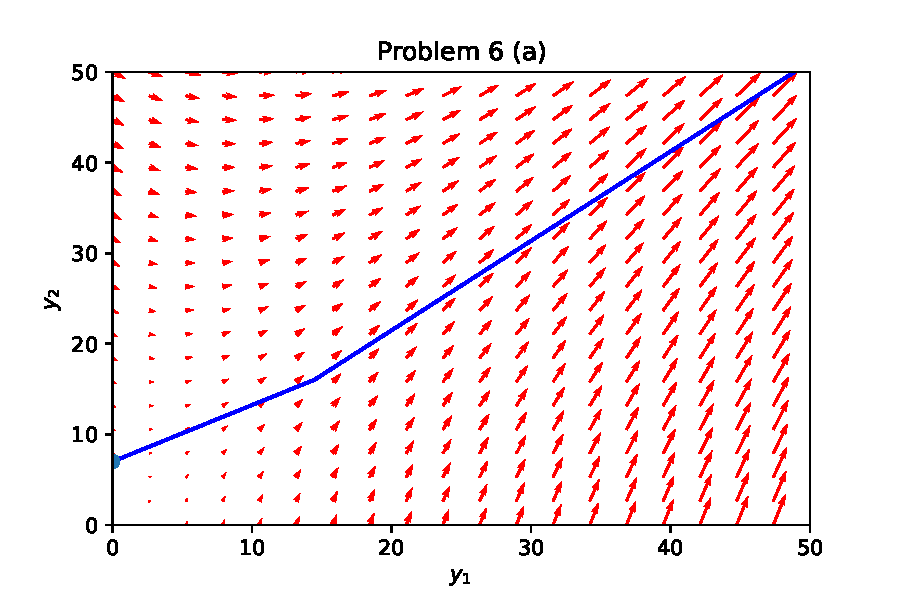
\includegraphics[width=0.49\textwidth]{6-(a).pdf}}} \hspace*{1mm}
    \subfloat[]{{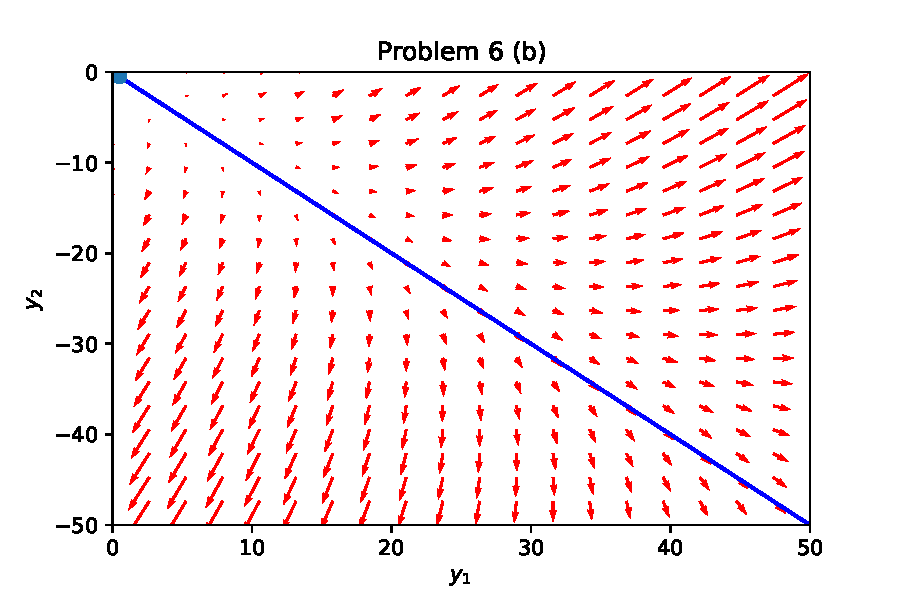
\includegraphics[width=0.49\textwidth]{6-(b).pdf}}}
\end{figure}


\end{document}